% Table in the shape of an arrow
% Author: Gonzalo Medina
\documentclass{article}
\usepackage{tikz}
\usetikzlibrary{calc,matrix,decorations.markings,decorations.pathreplacing}

\definecolor{colone}{RGB}{209,220,204}
\definecolor{coltwo}{RGB}{204,222,210}
\definecolor{colthree}{RGB}{207,233,232}
\definecolor{colfour}{RGB}{248,243,214}
\definecolor{colfive}{RGB}{245,238,197}
\definecolor{colsix}{RGB}{243,235,179}
\definecolor{colseven}{RGB}{241,231,163}

\tikzset{ 
  table/.style={
    matrix of nodes,
    row sep=-\pgflinewidth,
    column sep=-\pgflinewidth,
    nodes={rectangle,text width=2cm,align=center},
    text depth=1.25ex,
    text height=2.5ex,
    nodes in empty cells
  }
}

\renewcommand*{\familydefault}{\sfdefault}
\newcommand{\cbox}[1]{\parbox[t]{2cm}{\centering #1}}

\begin{document}

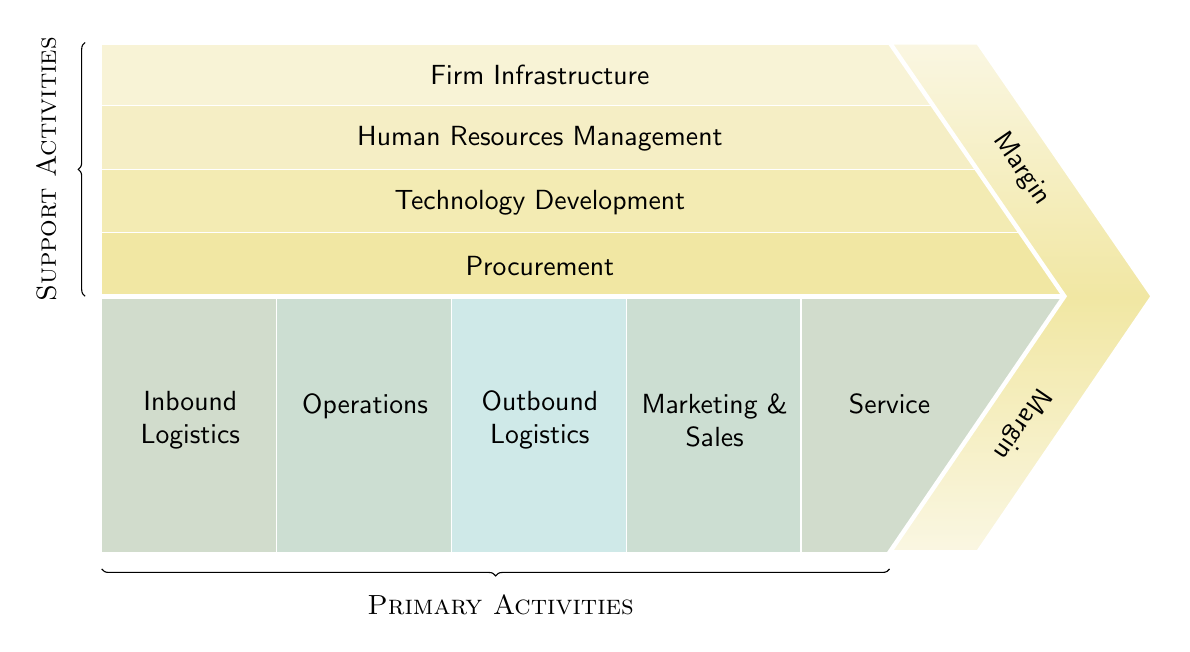
\begin{tikzpicture}
  \matrix (mat) [table] {
    |[fill=colfour]|      & |[fill=colfour]|  & |[fill=colfour]|
      & |[fill=colfour]|  & |[fill=colfour]|  &                   \\
    |[fill=colfive]|      & |[fill=colfive]|  & |[fill=colfive]|
      & |[fill=colfive]|  & |[fill=colfive]|  &                   \\
    |[fill=colsix]|       & |[fill=colsix]|   & |[fill=colsix]|
      & |[fill=colsix]|   & |[fill=colsix]|   & |[fill=colsix]|   \\
    |[fill=colseven]|     & |[fill=colseven]| & |[fill=colseven]|
      & |[fill=colseven]| & |[fill=colseven]| & |[fill=colseven]| \\
    |[fill=colone]|       & |[fill=coltwo]|   & |[fill=colthree]|
      & |[fill=coltwo]|   & |[fill=colone]|   & |[fill=colone]|   \\
    |[fill=colone]|       & |[fill=coltwo]|   & |[fill=colthree]|
      & |[fill=coltwo]|   & |[fill=colone]|   & |[fill=colone]|   \\
    |[fill=colone]|       & |[fill=coltwo]|   & |[fill=colthree]|
      & |[fill=coltwo]|   & |[fill=colone]|   &                   \\
    |[fill=colone]|       & |[fill=coltwo]|   & |[fill=colthree]|
      & |[fill=coltwo]|   & |[fill=colone]|   &                   \\
  };

  % horizontal rules
  \foreach \row in {2,3,4}
    \draw[white] (mat-\row-1.north west) -- (mat-\row-6.north east);
  \draw[white,ultra thick] (mat-1-1.north west) -- (mat-1-6.north east);
  \draw[white,ultra thick] (mat-5-1.north west) -- (mat-5-6.north east);

  % vertical rules
  \foreach \col in {2,3,4,5}
    \draw[white] (mat-5-\col.north west) -- (mat-8-\col.south west);

  % The labels
  \node[fill=colfour] at (mat-1-3) {Firm Infrastructure};
  \node[fill=colfive] at (mat-2-3) {Human Resources Management};
  \node[fill=colsix] at (mat-3-3) {Technology Development};
  \node[fill=colseven] at (mat-4-3) {Procurement};
  \node at ([yshift=-10pt]mat-6-1) {\cbox{Inbound Logistics}};
  \node at ([yshift=-10pt]mat-6-2) {\cbox{Operations \\\mbox{}}};
  \node at ([yshift=-10pt]mat-6-3) {\cbox{Outbound Logistics}};
  \node at ([yshift=-10pt]mat-6-4) {\cbox{Marketing \& Sales}};
  \node at ([yshift=-10pt]mat-6-5) {\cbox{Service \\\mbox{}}};
  \node[rotate = 90] at ([xshift=-52pt]mat-3-1.north)
    {\textsc{Support Activities}};
  \node at ([yshift=-19pt, xshift=-0.5cm]mat-8-3.south)
    {\textsc{Primary Activities}};

  % Erase some visible lines outside the arrow
  \fill[white] (mat-1-5.north east) -- (mat-5-6.north east)
    -- (mat-1-6.north east) -- cycle;
  \fill[white] (mat-8-5.north east) -- (mat-5-6.north east)
    -- (mat-8-6.north east) -- cycle;

  % Draw the arrow tip
  \shade[top color=colfour!70, bottom color=colfour!70,
    middle color=colseven, draw=white, ultra thick] 
    (mat-1-5.north) -- (mat-5-6.north) -- (mat-8-5.south) -- 
    (mat-8-5.south east) -- (mat-5-6.north east) -- (mat-8-5.south east) -- 
    (mat-5-6.north east) -- (mat-1-5.north east) -- cycle;

  % The slanted "Margin" labels
  \begin{scope}[decoration={markings,
    mark=at position .5 with \node[transform shape] {Margin};}]
  \path[postaction={decorate}] 
    ( $ (mat-1-5.north)!0.5!(mat-1-5.north east) $ )
    -- ( $ (mat-5-6.north)!0.5!(mat-5-6.north east) $ );
  \path[postaction={decorate}] 
    ( $ (mat-5-6.north)!0.5!(mat-5-6.north east) $ )
    -- ( $ (mat-8-5.south)!0.5!(mat-8-5.south east) $ );
  \end{scope}

  % The braces
  \draw[decorate, decoration={brace, mirror, raise=6pt}]
    (mat-1-1.north west) -- (mat-5-1.north west);
  \draw[decorate, decoration={brace, mirror, raise=6pt}]
    (mat-8-1.south west) -- (mat-8-5.south);
\end{tikzpicture}
\end{document}